\section{Results}
\label{sec:results}
On the SPI interface one should be able to successfully write and read back registers. Therefore a complete SPI driver was written in python which allows to simply mux out the wanted analog/digital signal, change the clock frequency and read back the register values. An overview of the registers can be found bellow \autoref{tab:reg_des} whereby register two does not exist as mentioned later on in \autoref{subsec:spi_register_offset}.
\subsection{SPI Interface}
\label{subsec:spi_interface}
\begin{longtable}{|p{3.5cm}|p{10.5cm}|}
	\hline
	\rowcolor{lightgray}
	\textbf{Register Number} &\textbf{Function} \\ \hline
	0 & stores the last spi command $<7:0>$\\ \hline
    1 & read only register with following value: b0=1, b1=0, b2=1, b3=0, b4=0, b5=0, b6=0, b7=0 <15:8> \\ \hline
    3 & analog mux $<20:16>$ 0=ground, 1=iboot ref, 2=vbgp, 3=output error amplifier, 4=ground,  5= ground \\ \hline
	4 & current limit tune $<27:25>$, current limit tune enable $<24>$ \\ \hline
	5 & output voltage fb $<32>$ \\ \hline
	6 & Freq tune digital part $<42:40>$ can add up to 3 caps eq sized caps to saw tooth ==> clock 4 times slower, dig out$<47>$ ==> enable clock on digital pad\\ \hline
    7 & Freq tune linear regulator$<50:48>$ can add up to 3 caps eq sized caps to saw tooth ==> clock 4 times slower \\ \hline
	\caption{Register description} % needs to go inside longtable environment
	\label{tab:reg_des}
\end{longtable}
Since the the SPI communication is working as in the testbench and the testscript is available in the git repository. No further test results are listed here. But one thing that one has to be aware of when one wants to control the chip is that the CS line has to be activated before the first clock edge arrives otherwise the communication will not work as mentioned in \autoref{subsubsec:SPI}.

\subsection{POR}
According to the simulation, the power-on reset (POR) exhibits the characteristics depicted in \autoref{tab:por}. The POR measurement was conducted on a single random sample at room temperature. To measure the characteristics from the simulation, a pull-up resistor was connected to the output of the analog test pin as the test pin exhibits high impedance when the chip is unpowered and is grounded when the chip is powered (as long as the analog test pint was not configured differently over the SPI).
Consequently, when the chip gets powered and reaches a voltage over the minimum voltage of the POR, the analog test pin is driven to zero and this change is observable. Due to that it turned out that the minimum voltage of the POR is \qty{3.72}{\volt} which is \qty{0.02}{\volt} more than the upper corner of the Simulation. Since the time was limited and the deviation is very small no further investigations were made on that. The input and output delay where measured the same way and it turned out that those values are inside the corners of the simulations. For the input delay a value of \qty{40}{\micro\second} was measured which is the time from which the input voltage is over over  \qty{3.72}{\volt} and the analog test pin is driven to ground. The other way around a value of \qty{6.5}{\micro\second} was measured as it can be also seen in \autoref{tab:por} column four.
\begin{longtable}{|p{5cm}|p{2cm}|p{2cm}|p{2cm}|p{2cm}|}
	\hline
	\rowcolor{lightgray}
	\textbf{Description} &\textbf{Min.} &\textbf{Max.} & \textbf{Mes.} & \textbf{Unit} \\ \hline
	
	Input Delay & 26 & 44 & 40  &\qty{}{\micro\second} \\ \hline
	Output Delay & 4.4 & 6.8 & 6.5 &\qty{}{\micro\second} \\ \hline
	Current Consumption & 13 & 31 & -& \qty{}{\micro\ampere} \\ \hline
	Min Voltage & 3.176& 3.7 & 3.72 & \qty{}{\volt} \\ \hline
	\caption{POR characteristic} % needs to go inside longtable environment
	\label{tab:por}
\end{longtable}
\subsection{Bandgap}
\label{subsubsec:bandgap}
The bandgap characteristics from the simulation can be seen in \autoref{tab:bandgap}, \autoref{fig:bandgap_voltage_vs_temp} and \autoref{fig:bandgap_voltage_mc}. The measurements have thereby shown that the bandgap voltage is in the range of of the simulation, the mean value is just shifted by 10mV. As it can be seen in the comparison of \autoref{fig:bandgap_voltage_distrb} and \autoref{fig:bandgap_voltage_mc}. Furthermore due to the fact that the reference current is slightly to high the center of the bandgap vs temperature curve is not anymore at \qty{40}{\degreeCelsius} but at about \qty{55}{\degreeCelsius} as it can be seen in the comparison of \autoref{fig:bandgap_voltage_vs_temp} and \autoref{fig:bandgap_voltage_vs_temp_mes}. About the other parameters like the current consumption and the min voltage no measurements could be done since the band gap is not directly accessible.
\begin{longtable}{|p{5cm}|p{2.5cm}|p{2.5cm}|p{2.5cm}|}
	\hline
	\rowcolor{lightgray}
	\textbf{Description} &\textbf{Min} &\textbf{Max} & \textbf{Unit} \\ \hline
	
	Bandgap Voltage & 1.226 & 1.277 &\qty{}{\volt} \\ \hline
	Current Consumption & 16.73 & 23.53 & \qty{}{\micro\ampere} \\ \hline
	Min Voltage & 2.3& 2.9 & \qty{}{\volt} \\ \hline
	\caption{Bandgap characteristic} % needs to go inside longtable environment
	\label{tab:bandgap}
\end{longtable}
\begin{figure}[ht]
	\centering
	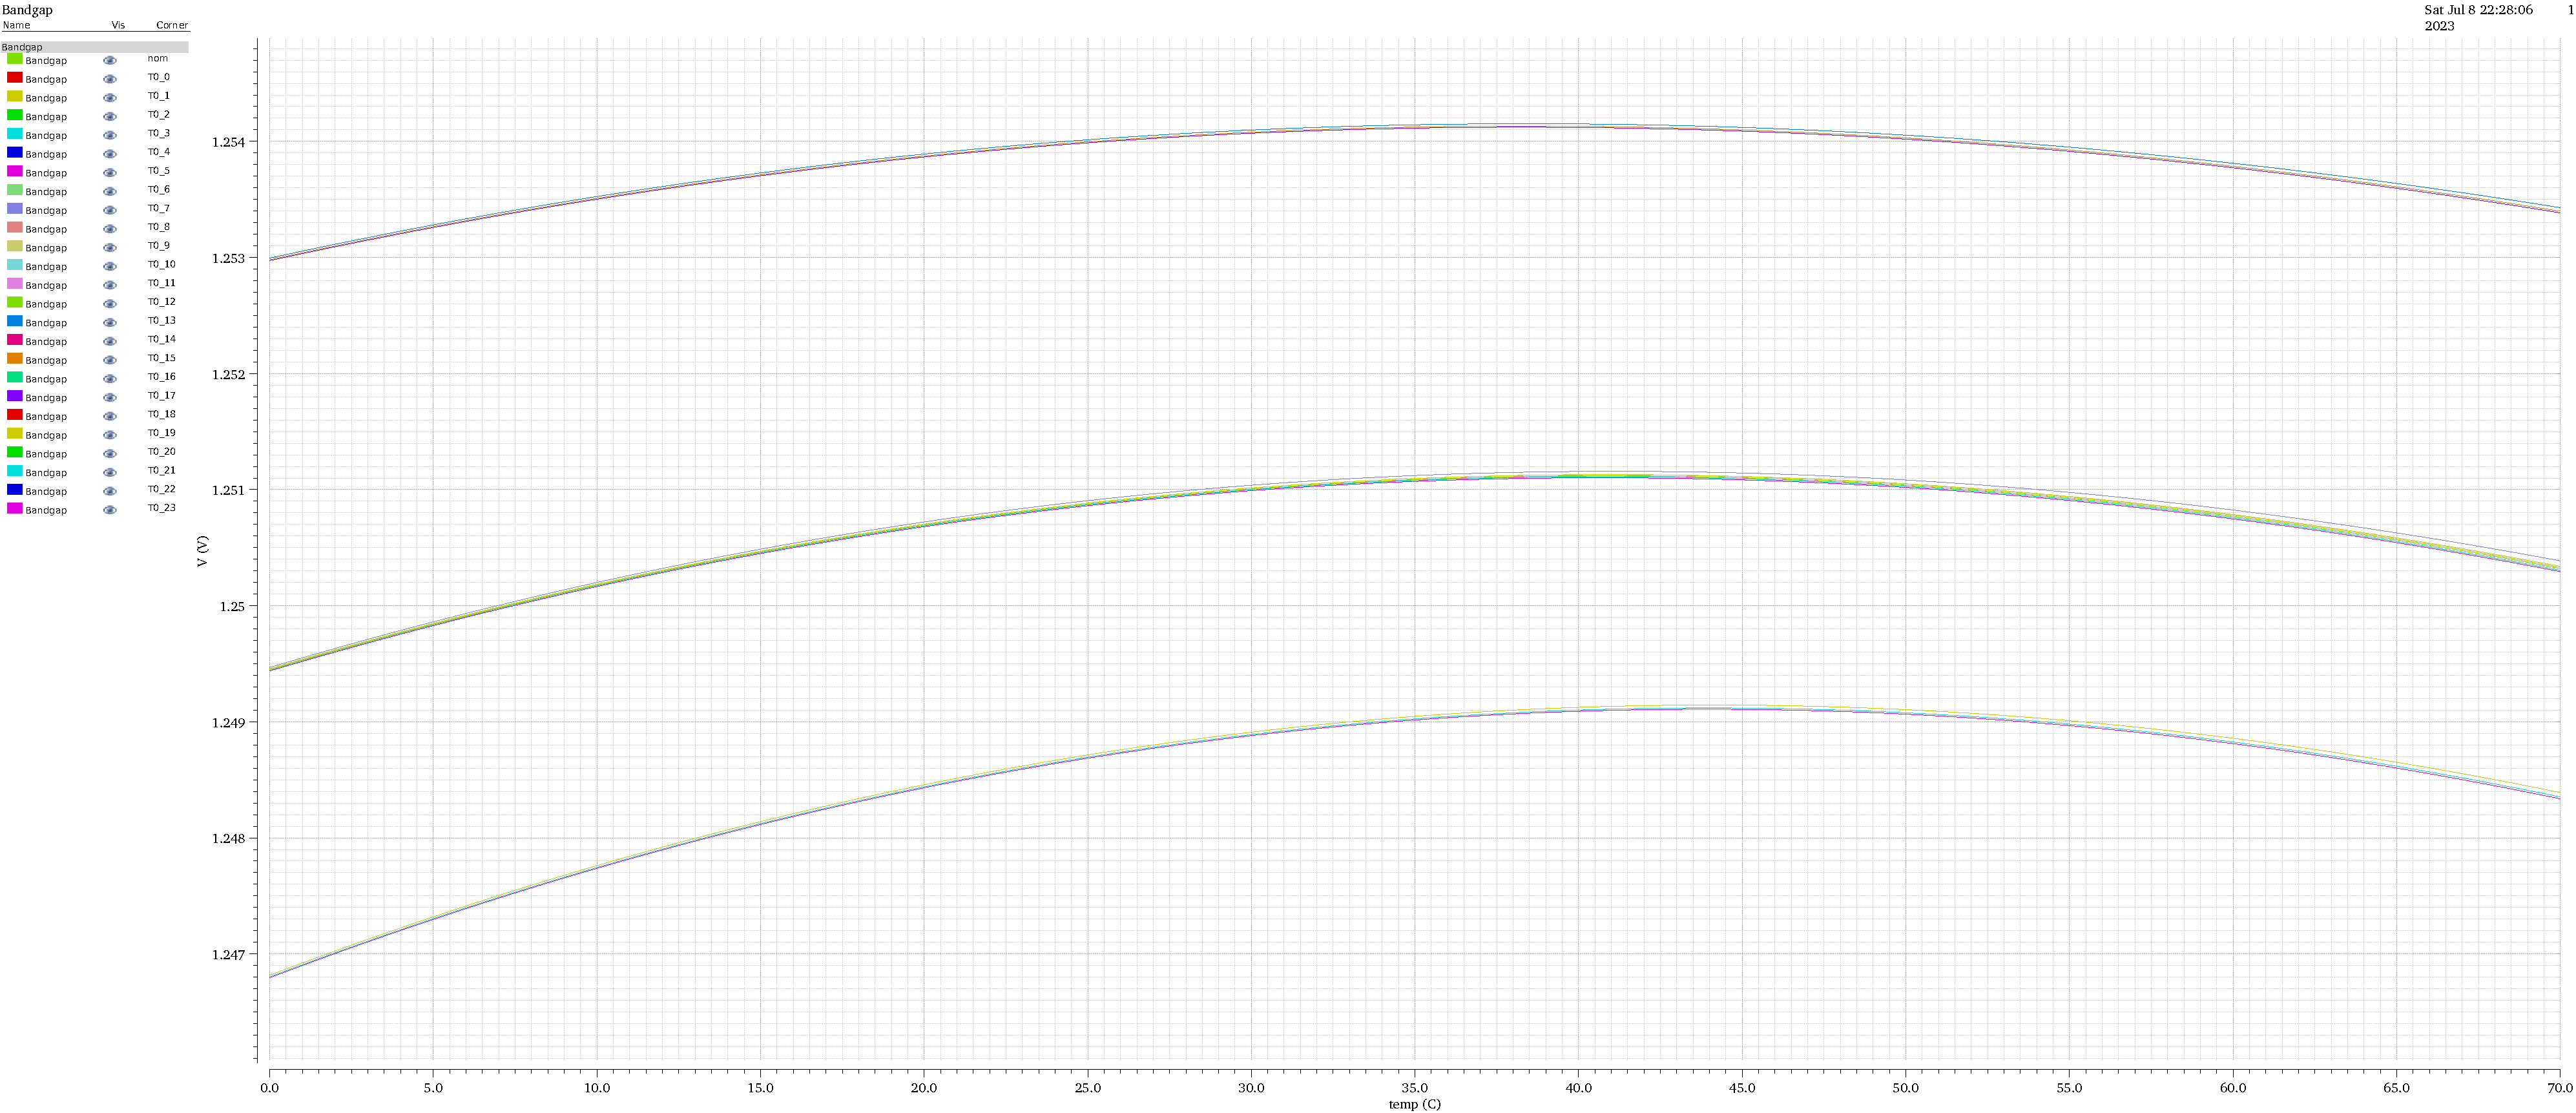
\includegraphics[width=\textwidth]{images/05_bandgap/band_volt.pdf}
	\caption{Bandgap voltage vs temperature simulated}
	\label{fig:bandgap_voltage_vs_temp}
\end{figure}
\begin{figure}[ht]
	\centering
	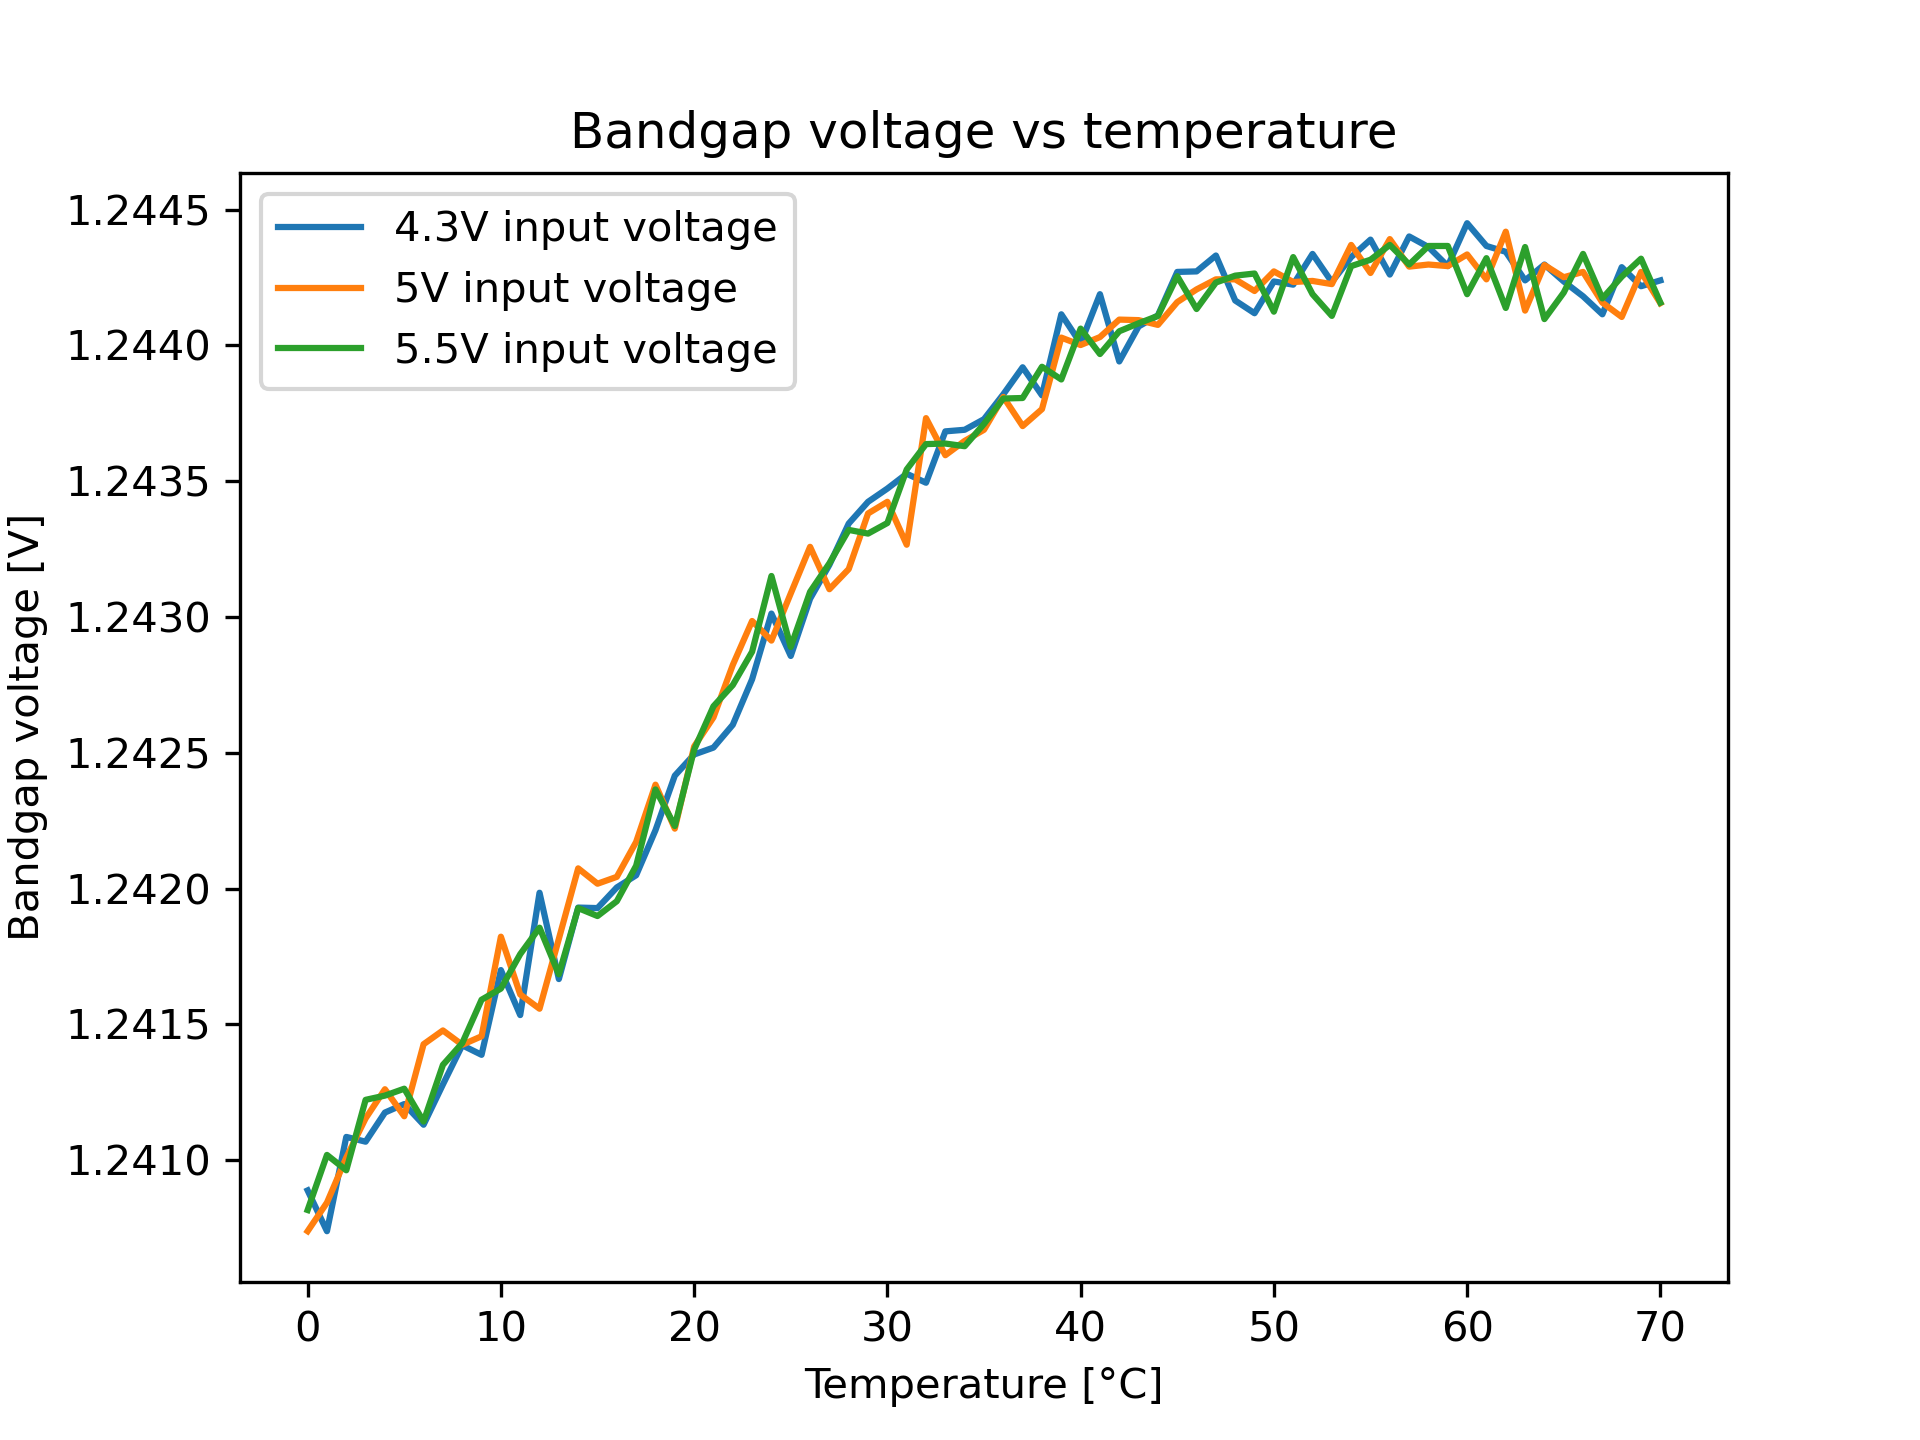
\includegraphics[width=\textwidth]{images/05_bandgap/Bandgap.png}
	\caption{Bandgap voltage vs temperature measured}
	\label{fig:bandgap_voltage_vs_temp_mes}
\end{figure}
\begin{figure}[ht]
	\centering
	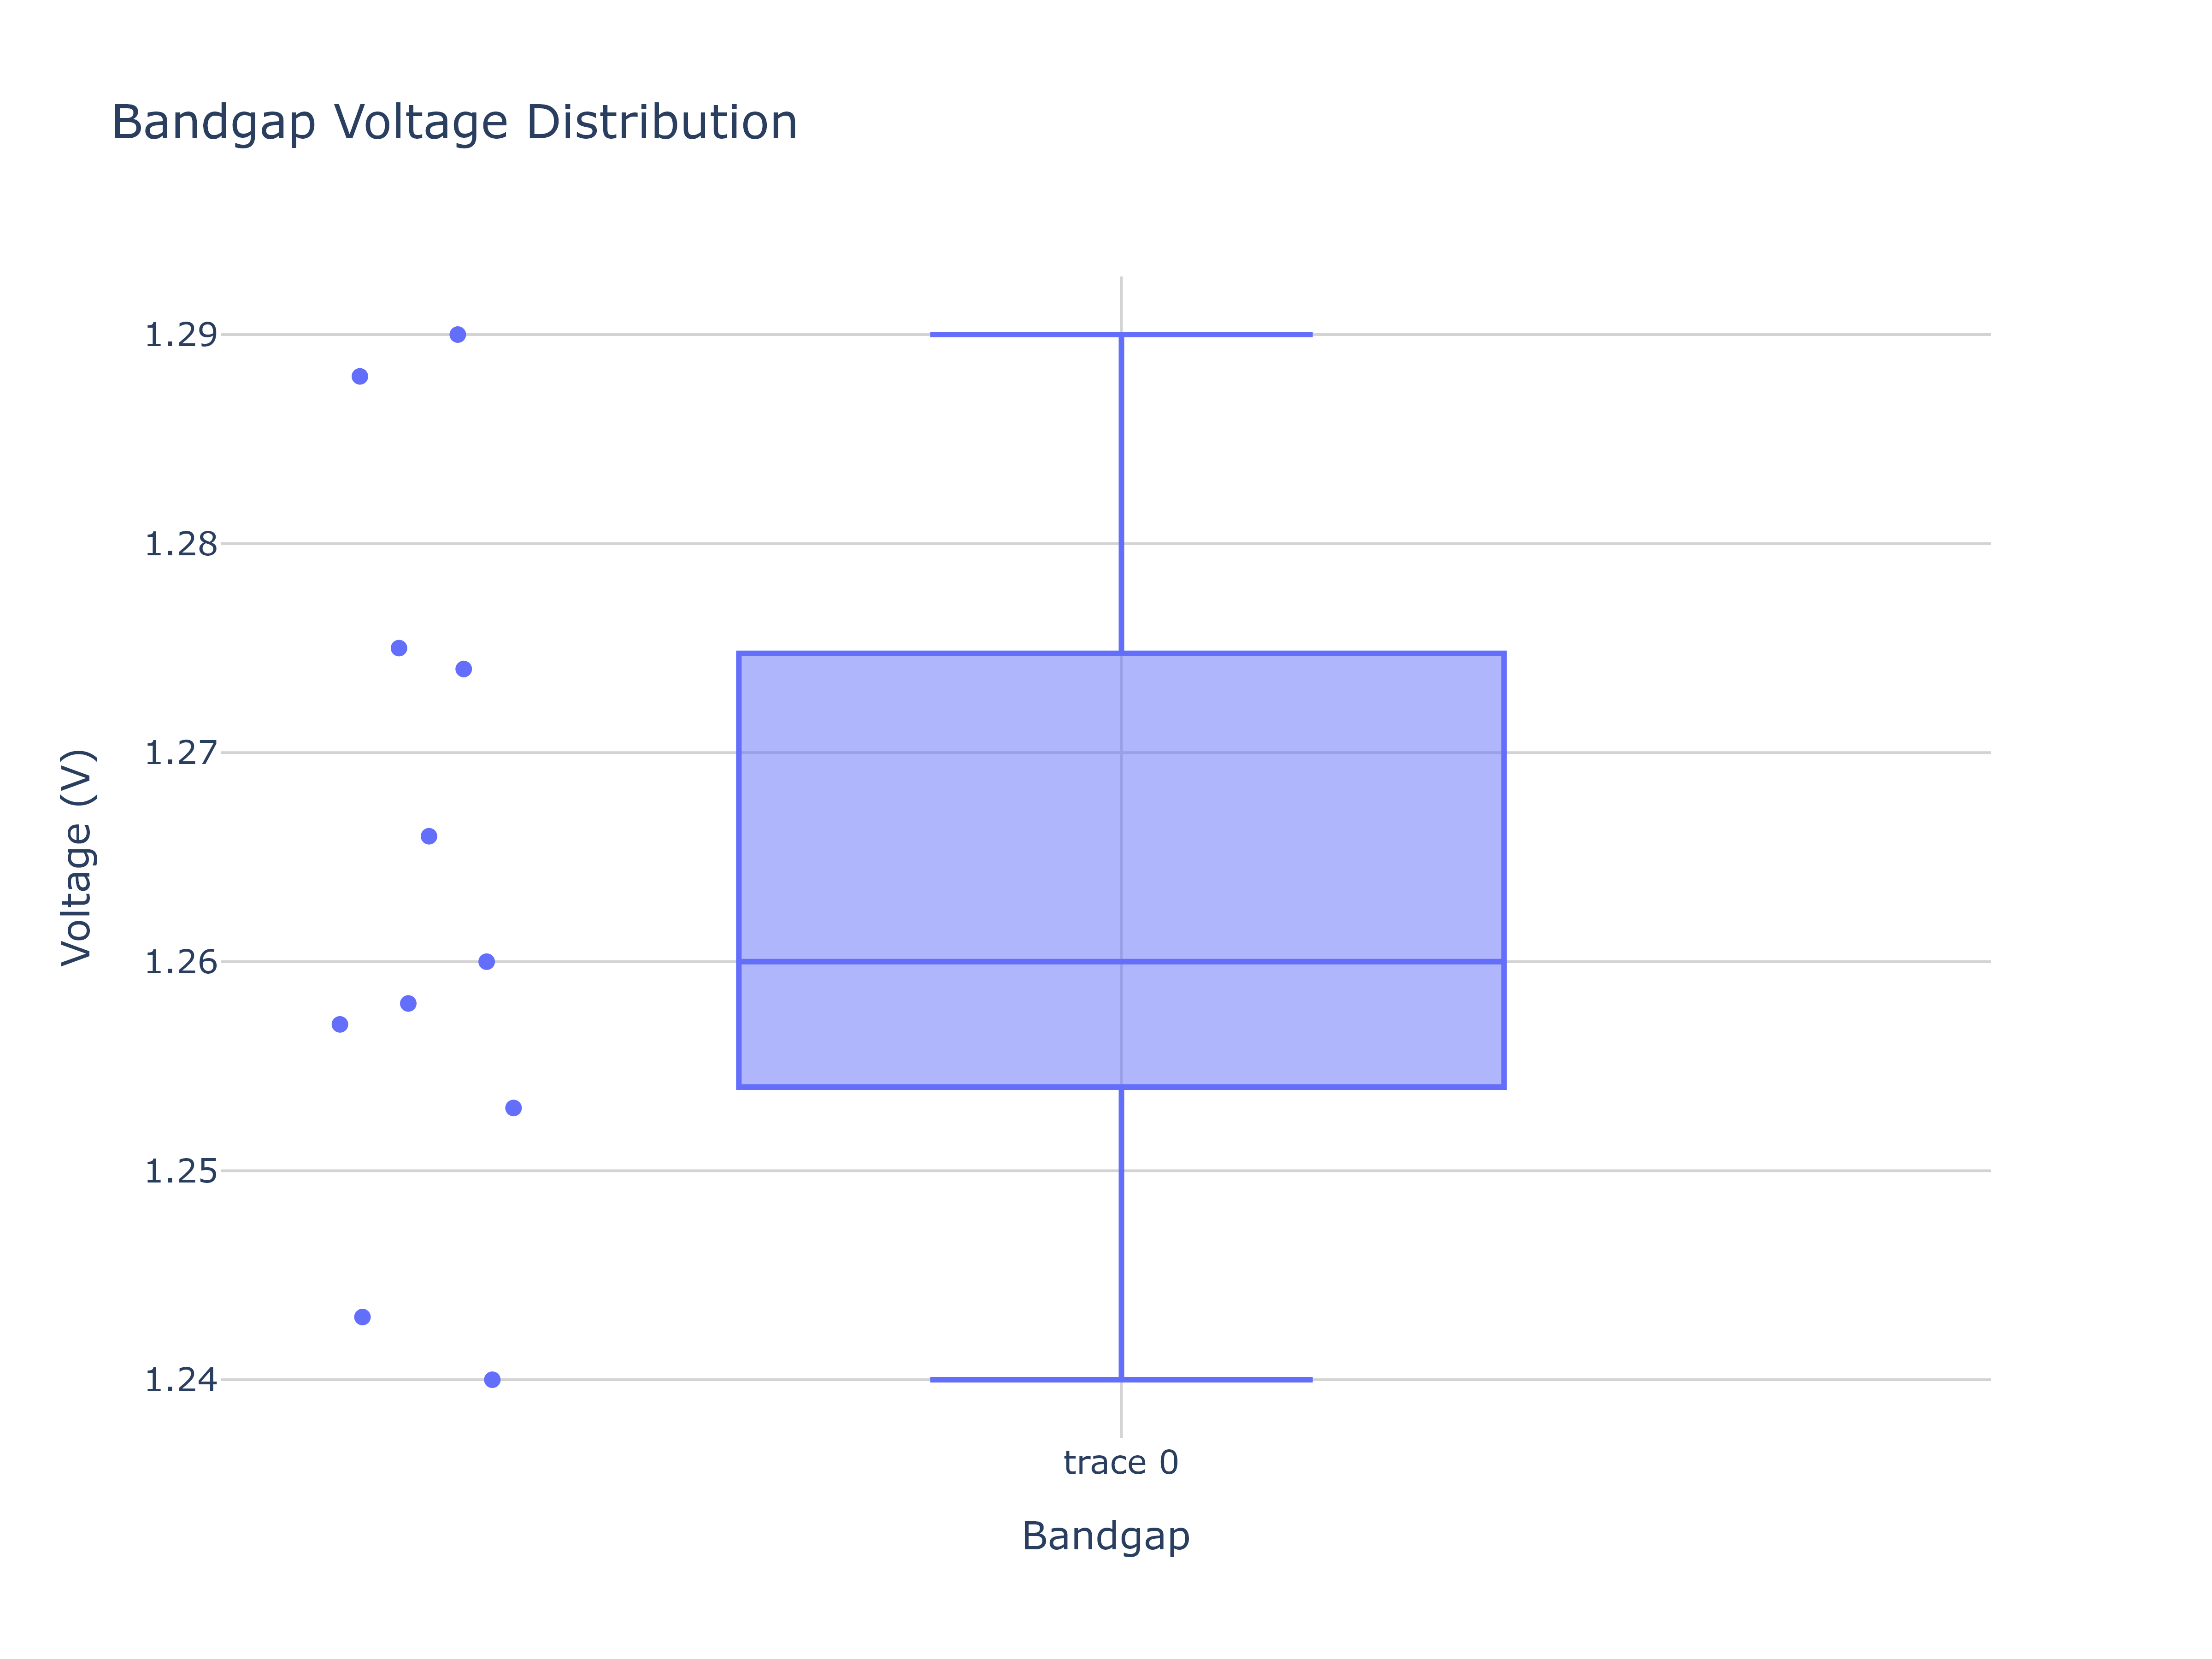
\includegraphics[width=\textwidth]{images/Bandgap_Voltage_Distribution.png}
	\caption{Bandgap voltage distribution at \qty{22}{\degreeCelsius} and 5V}
	\label{fig:bandgap_voltage_distrb}
\end{figure}

\begin{figure}[ht]
	\centering
	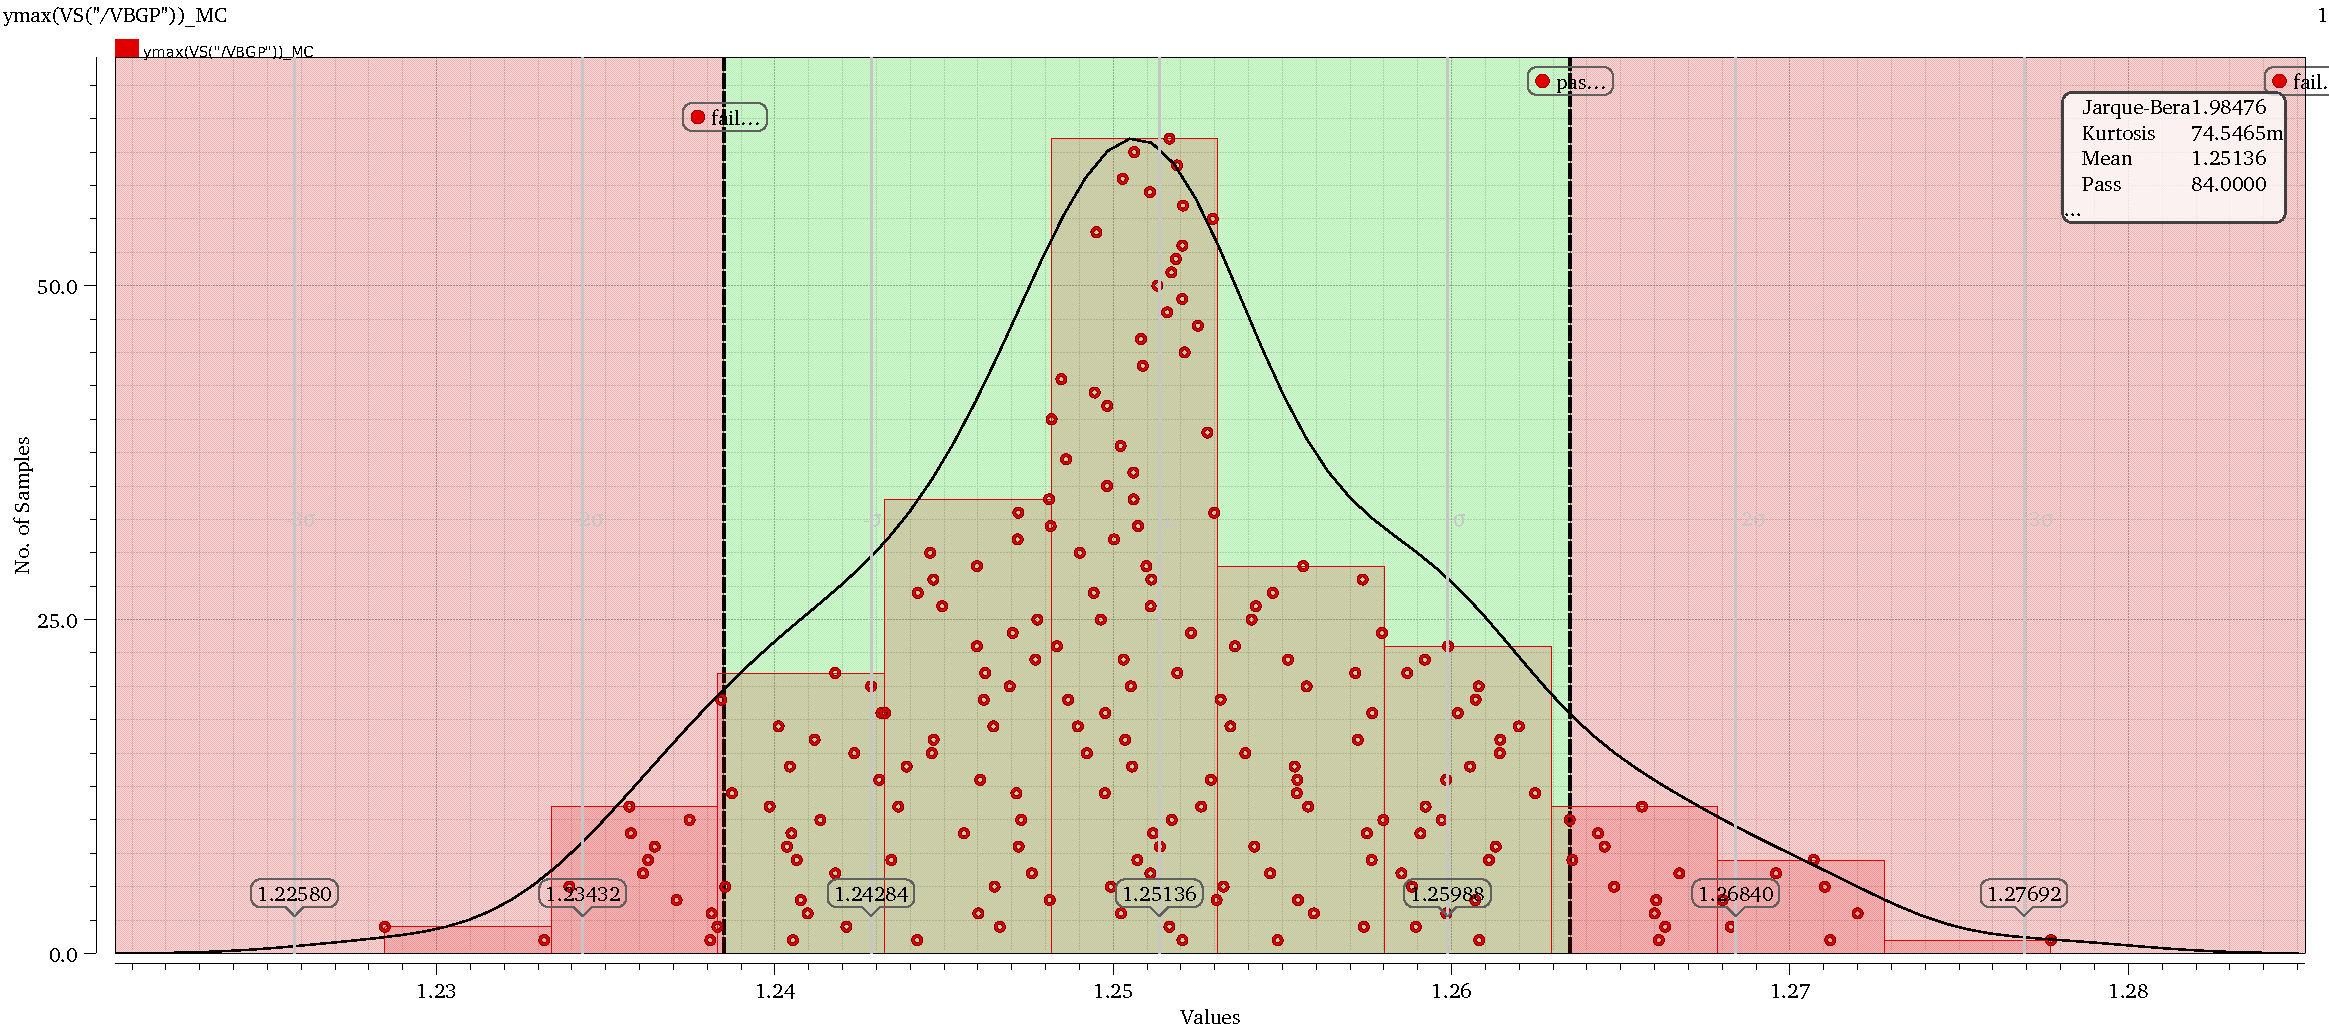
\includegraphics[width=\textwidth]{images/05_bandgap/band_volt_mc.pdf}
	\caption{Bandgap voltage Monte Carlo simulation (param.scs=3s, xh035.scs=mcg)}
	\label{fig:bandgap_voltage_mc}
\end{figure}
\clearpage
\subsection{Current Source}
\label{subsubsec:current_source}
The current source characteristics from the simulation can be seen in \autoref{tab:current_source} and \autoref{fig:ref_cur_mont}. The measurements have thereby shown that the current source is not in the range of the simulation. The current measured is about \qty{4}{\micro\ampere} higher than the one simulated which corresponds to a deviation of $\left|\frac{\qty{14.3}{\micro\ampere}-\qty{10.3}{\micro\ampere}}{\qty{10.3}{\micro\ampere}}\right|\cdot 100\approx 38.8 \%$. An exact explanation for this behavior was not found, but since the oscillator has a similar deviation and is independently of the current source the deviation most probably comes from the \glqq rmp1\grqq{} resistors since those were used in the layout of the oscillator and the current reference.
The current measured can be seen in \autoref{fig:current_source_distr}. About the other parameters no measurements could be done since the current source is not directly accessible.
\begin{longtable}{|p{5cm}|p{2.5cm}|p{2.5cm}|p{2.5cm}|}
	\hline
	\rowcolor{lightgray}
	\textbf{Description} &\textbf{Min} &\textbf{Max} & \textbf{Unit} \\ \hline
	
	Reference Current & 8.4 & 13.5 &\qty{}{\micro\ampere} \\ \hline
	Current Consumption & 50 & 81 & \qty{}{\micro\ampere} \\ \hline
	Min Voltage (Threshold where $\frac{\Delta V_{in}}{\Delta I_{out}}$ > \qty{1}{\mega\ohm}) & 3& 3.33 & \qty{}{\volt} \\ \hline
	\caption{Current reference characteristics} % needs to go inside longtable environment
	\label{tab:current_source}
\end{longtable}
\begin{figure}[ht]
	\centering
	\resizebox{1\textwidth}{!}{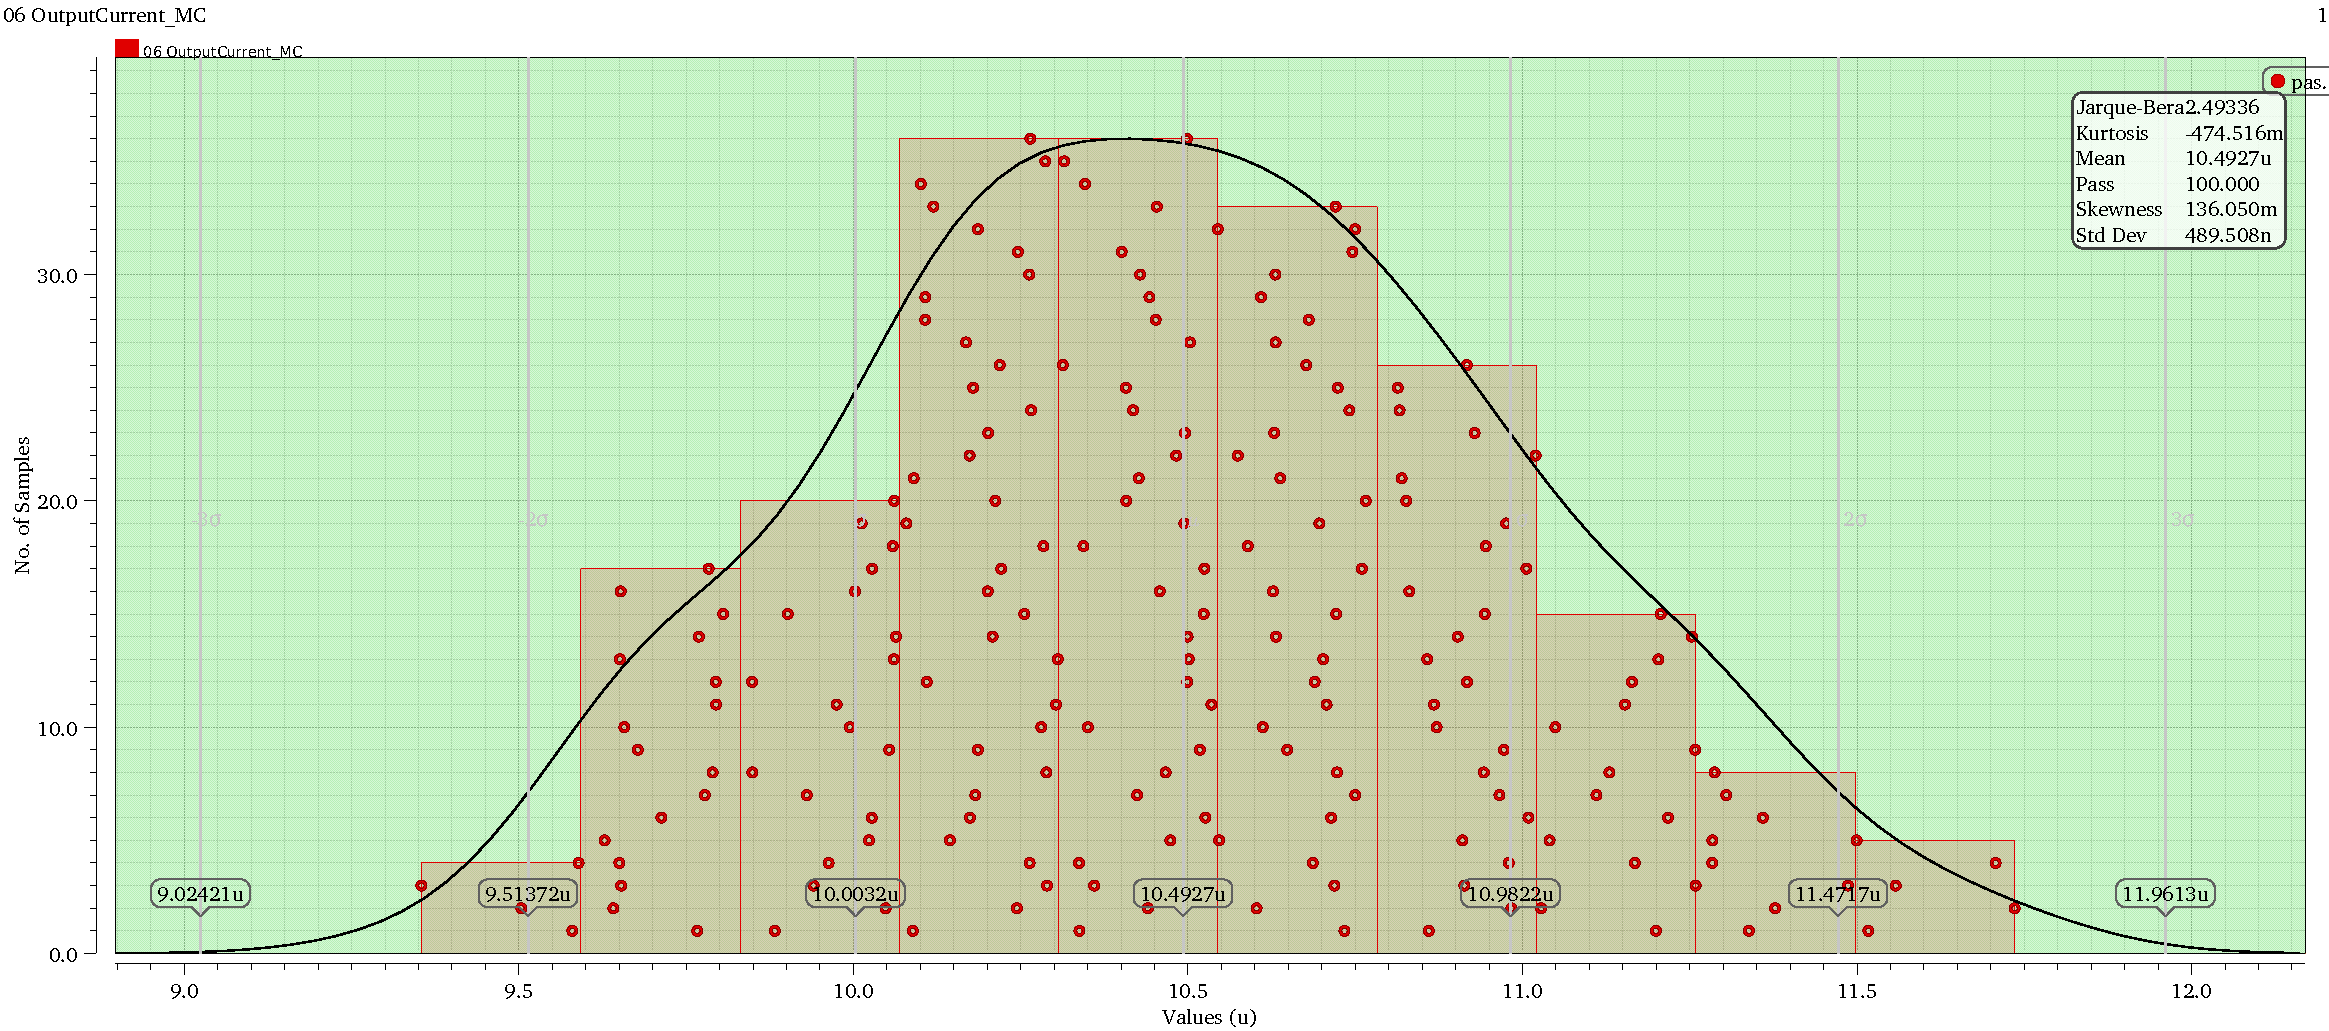
\includegraphics{images/06_current_ref/ref_cur_mont.pdf}}
	\caption{Monte Carlo distribution of Current reference. X-axis shows current through \glqq IPRB0\grqq{} in \autoref{fig:ref_cur_sim_schem} (param.scs=3s, xh035.scs=mcg)}
	\label{fig:ref_cur_mont}
\end{figure}
\begin{figure}[ht]
	\centering
	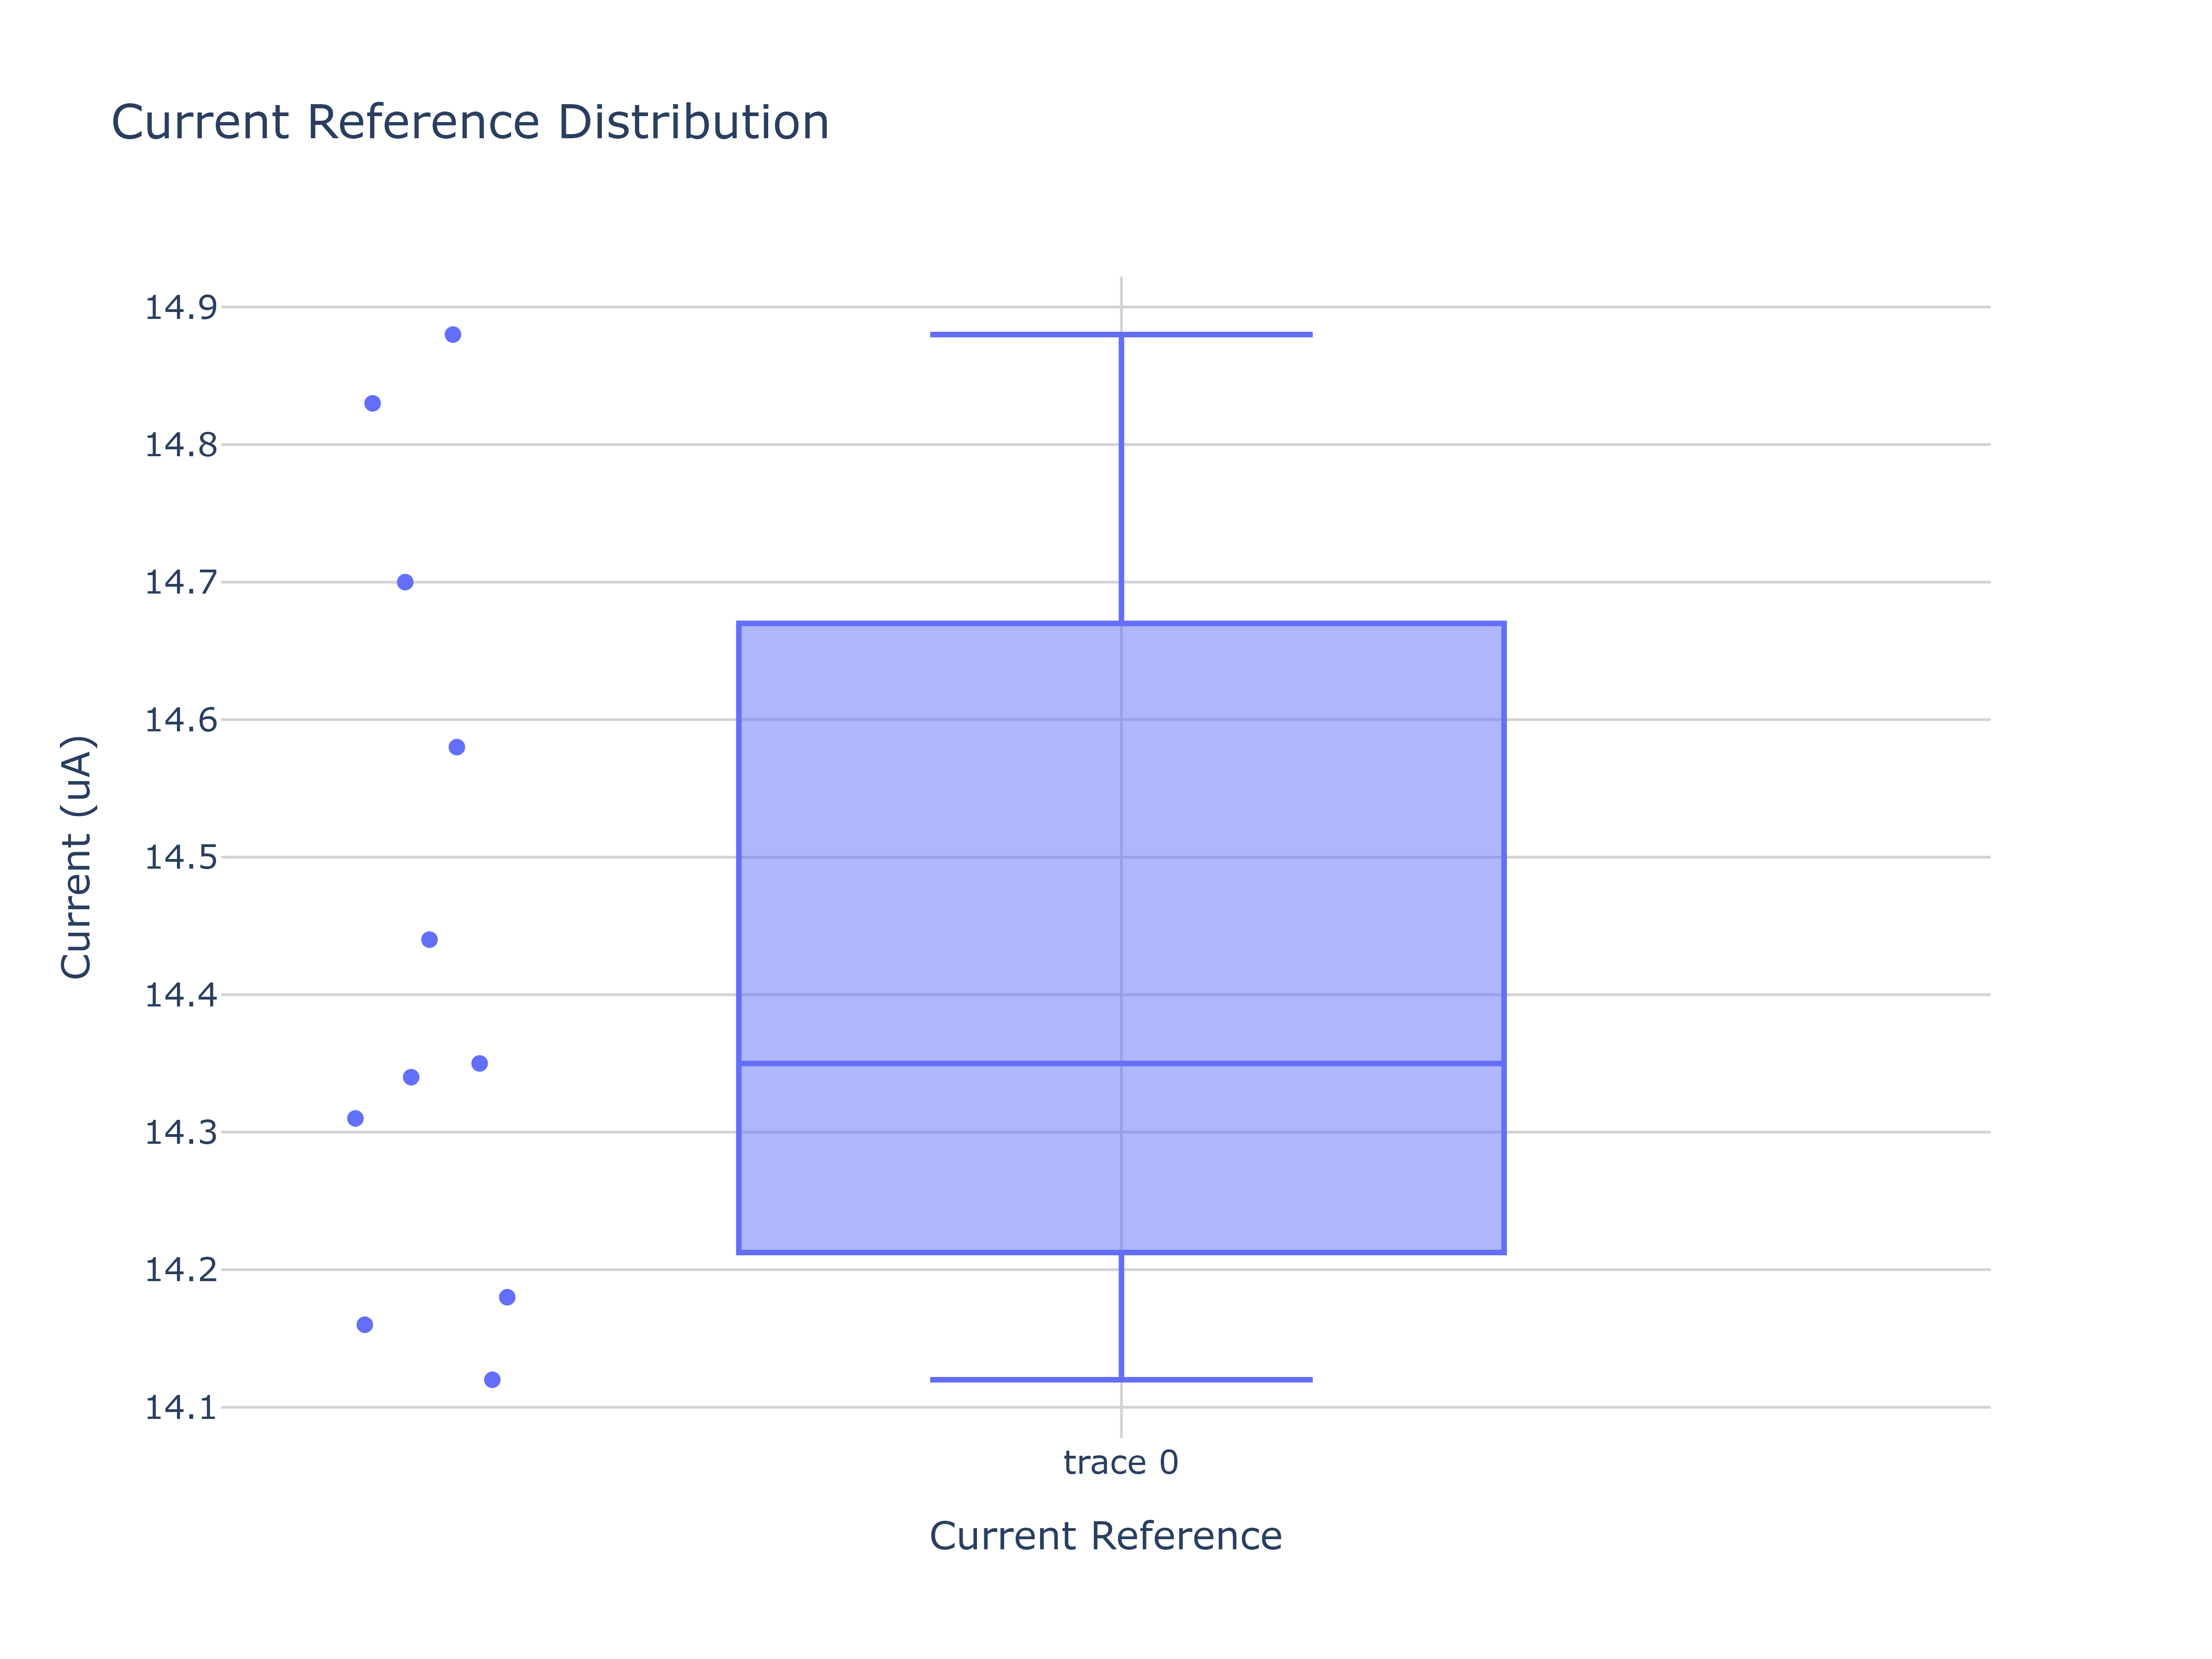
\includegraphics[width=\textwidth]{images/Current_Reference_Distribution.png}
	\caption{Current source distribution at \qty{22}{\degreeCelsius} and 5V}
	\label{fig:current_source_distr}
\end{figure}
\clearpage
\subsection{Oscillator}
\label{subsubsec:oscillator}
The oscillator characteristics from the simulation can be seen in \autoref{tab:osc}. The measurements have thereby shown that the oscillator is not in the range of of the simulation, when there is no configuration made over the SPI one has a nominal frequency of \qty{2.63}{\mega\hertz}, whereas in the simulation one had \qty{1.7}{\mega\hertz}, which results in an deviation of $\left|\frac{\qty{2.63}{\mega\hertz}-\qty{1.7}{\mega\hertz}}{\qty{1.7}{\mega\hertz}}\right|\cdot 100\approx 54.7 \%$, which is even more than in the current reference circuit. About the other parameters no measurements could be done since the oscillator is not directly accessible. Furthermore the frequency can also be tuned in the range of \qty{1.17}{\mega\hertz} to \qty{2.63}{\mega\hertz} over the spi registers (measured values) which results in the frequencies which can be seen in \autoref{tab:freq}. 
\begin{longtable}{|p{5cm}|p{2.5cm}|p{2.5cm}|p{2.5cm}|}
	\hline
	\rowcolor{lightgray}
	\textbf{Description} &\textbf{Min} &\textbf{Max} & \textbf{Unit} \\ \hline
	
	Frequency & 1.15 & 1.8 &\qty{}{\mega\hertz} \\ \hline
	Current Consumption & 35 & 50 & \qty{}{\micro\ampere} \\ \hline
	Min Voltage & 2& 3.187 & \qty{}{\volt} \\ \hline
	\caption{Oscillator specification} % needs to go inside longtable environment
	\label{tab:osc}
\end{longtable}
\begin{table}[h]
	\centering
	\begin{tabular}{|c|c|}
		\hline
		\rowcolor{lightgray}
		\textbf{Register configuration} & \textbf{Frequency (kHz)} \\
		\hline
		0 & \qty{2630}{} \\
		\hline
		1 & \qty{2300}{} \\
		\hline
		2 & \qty{2190}{}\\
		\hline
		3 & \qty{1850}{} \\
		\hline
		4 & \qty{1670}{} \\
		\hline
		5 & \qty{1430}{}\\
		\hline
		6 & \qty{1270}{} \\
		\hline
		7 & \qty{1170}{}\\
		\hline
	\end{tabular}
	\caption{Measured frequency with different register configurations at \qty{22}{\degreeCelsius} and \qty{5}{\volt}}
	\label{tab:freq}
\end{table}


\clearpage


\subsection{Buck-Boost Converter}

\subsubsection{Start-up}
\label{sec:startup}
The start-up behavior shows significant differences to the results observed in simulations. Instead of the expected gradual increase in the output voltage, we observed the output voltage increase in distinct steps as can be seen in \autoref{fig:startup}. These distinct steps stem from the fact the input voltage collapses cyclicly to under the limit given by the \ac{POR}. The cycle can be described as the chip starting up and increasing the input current until the input voltage drops to bellow the limit given by the \ac{POR} thus disabling the chip and causing the input voltage to rise until the chip starts up again. The cycle continues until the output voltage reaches close to the nominal level and the outer voltage control loop regulates the current.  
The underlying issue is a misconfiguration of the internal registers causing the current limit to be disabled on start-up and the converter increasing the inductor current $I_L$ to unsustainable levels leading to the collapse of the input voltage. The cause is further described in \autoref{sec:missingcurrentlimit}.

\begin{figure}[ht]
	\centering
	
	\resizebox{1\textwidth}{!}{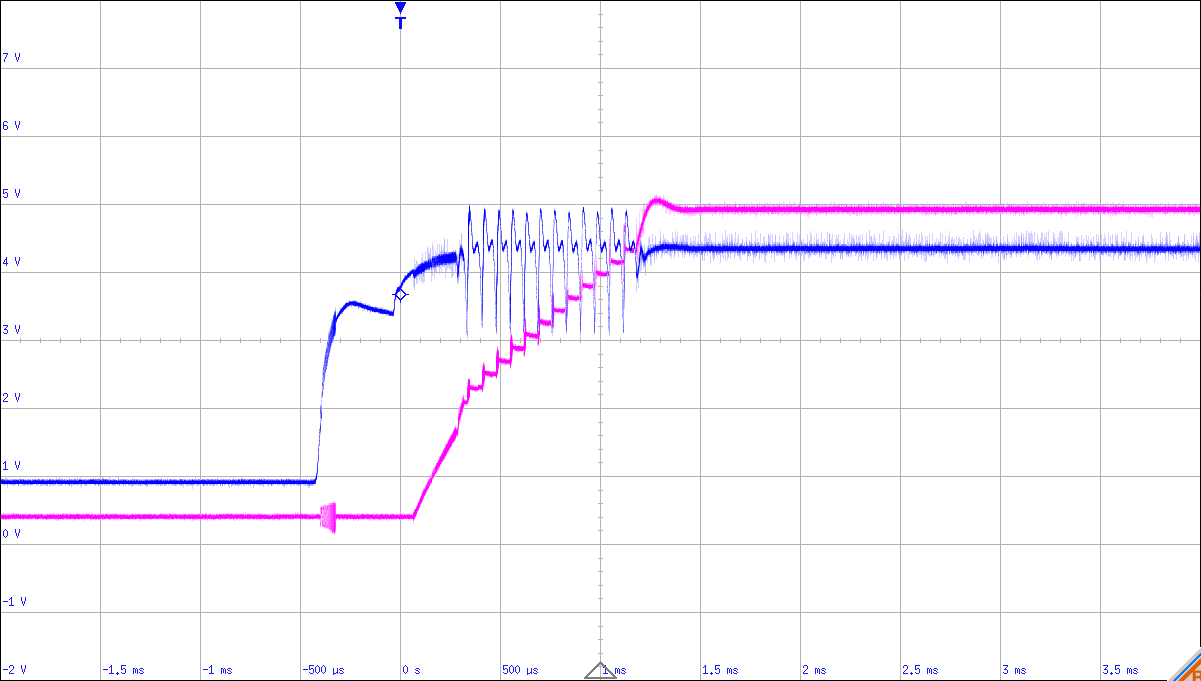
\includegraphics{images/07_DCDC/StartUp.PNG}}
	\caption{Start-up behavior without an attached load. Dark Blue: $V_{IN}$ measured; Pink: $V_{OUT}$ measured}
	\label{fig:startup}
\end{figure}
\clearpage


\subsubsection{Load Step Response}
The response to a load step is satisfactory and can be seen \autoref{fig:loadstep}. The regulation behavior is similar to the simulated response, but the measured controller has a higher bandwidth as can be seen in the faster response and is slightly overcompensated as it lacks the single oscillatory peak seen in the simulated response. Based on this response we estimate the implemented system has the following characteristics:

\begin{table}[H]
    \centering
    \begin{tabular}{|c|c|c|}
        Characteristic & Measured System & Simulation \\
        \hline
         Phase Margin  & \qty{55}{\degree} & \qty{45}{\degree}\\
		 Crossover Frequency & \qty{30}{\kilo\hertz} & \qty{20}{\kilo\hertz}  \\
    \end{tabular}
    \caption{Estimated regulator characteristics based on the response to a 200 mA load step}
    \label{tab:regChar}
\end{table}

\begin{figure}[ht]
	\centering
	
	\resizebox{1\textwidth}{!}{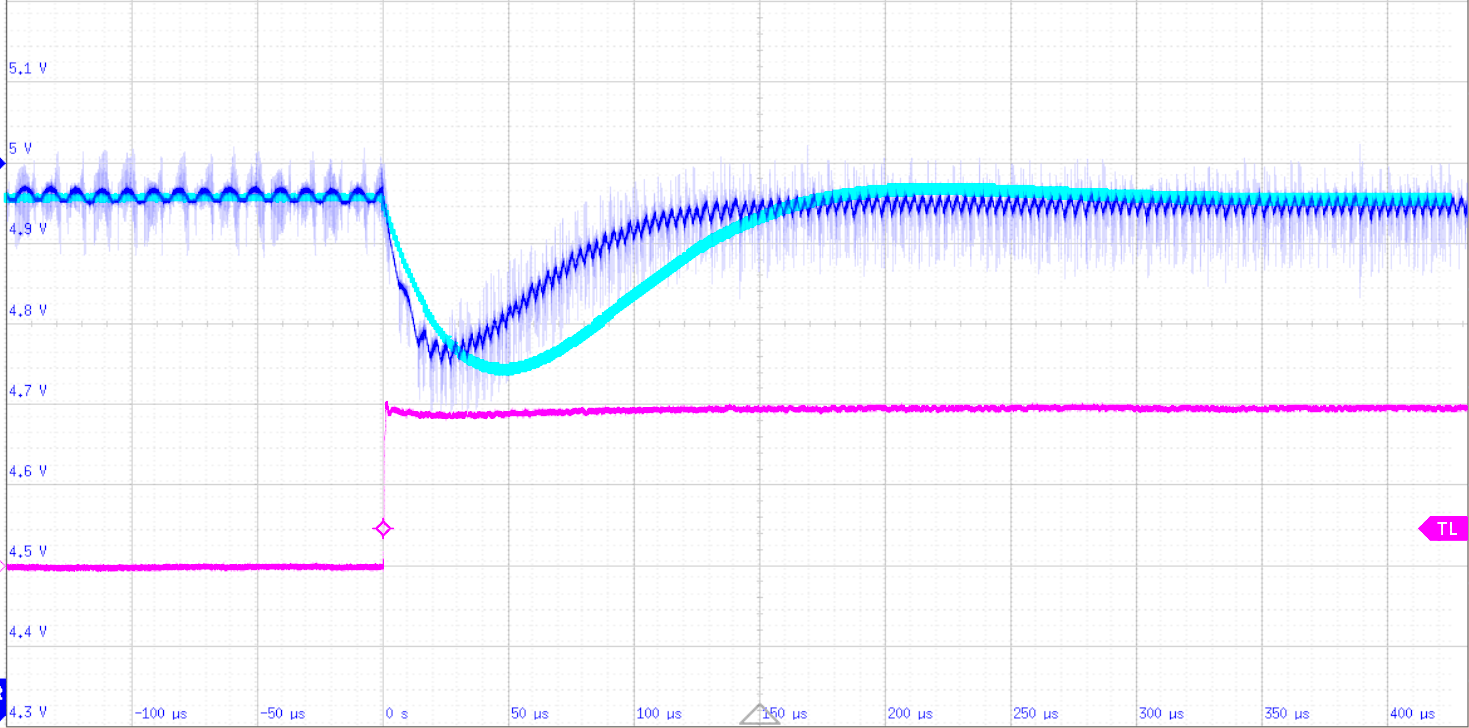
\includegraphics{images/07_DCDC/LoadStepVergleich.png}}
	\caption{Load regulation to a 200 mA load step for comparison between measured response and simulated response. Simulated response offset to remove constant load regulation error. Dark Blue: $V_{OUT}$ measured; Light Blue: $V_{OUT}$ simulated; Pink: $I_{OUT}$ measured}
	\label{fig:loadstep}
\end{figure}
\clearpage

\subsubsection{Load Regulation}
\label{sec:loadRegulation}
\begin{figure}[ht]
	\centering
	\resizebox{0.8\textwidth}{!}{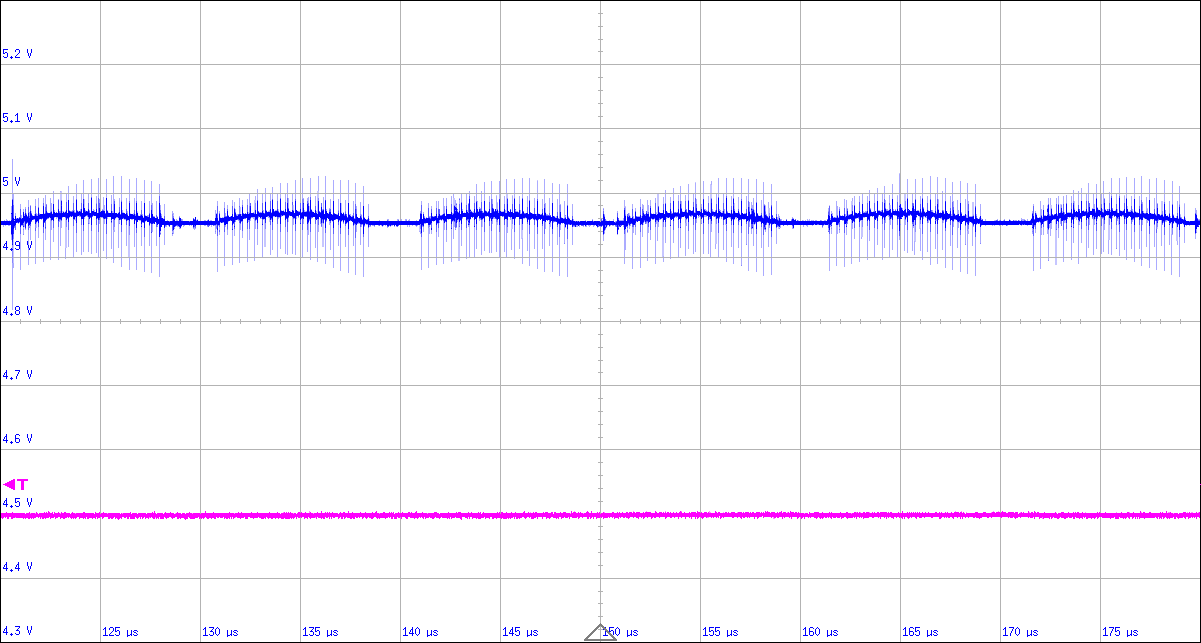
\includegraphics{images/07_DCDC/LoadSteadyState0mA.png}}
	\caption{Steady state load regulation with a 0mA load. Dark Blue: $V_{OUT}$; Pink: $I_{OUT}$}
\end{figure}
\begin{figure}[ht]
	\centering
	\resizebox{0.8\textwidth}{!}{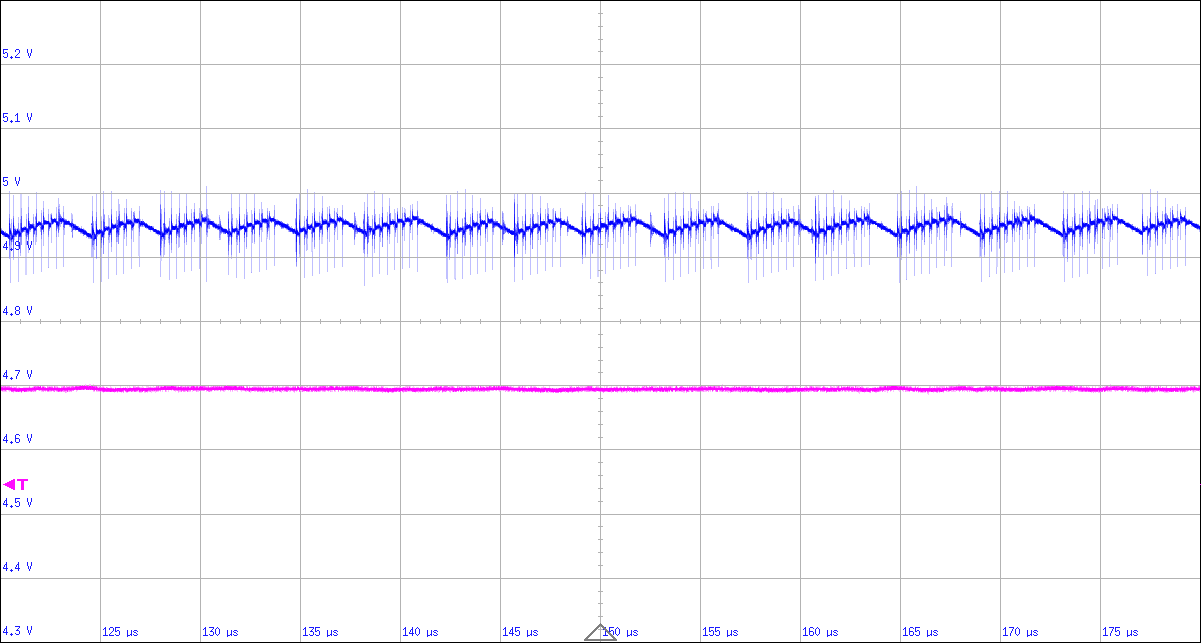
\includegraphics{images/07_DCDC/LoadSteadyState200mA.png}}
	\caption{Steady state load regulation with a 200mA load. Dark Blue: $V_{OUT}$; Pink: $I_{OUT}$}
\end{figure}
\clearpage



%\foreach \i in {../ASIC-DESIGN-2/images/03_plots/DCDC Reset Test with 4.3V and resistor R2\, 70°C} {
%    \begin{figure}[h]
%        \centering
%    \includegraphics[width=0.95\textwidth]{\i.pdf}
%    %     \caption{\i}
%    \end{figure}
%    
%}
\subsubsection{Efficiency}
\label{sec:efficiency}
%The efficiency of the TI chip was measured at different input voltages and loads. The efficiency was thereby callculated by difiding the output power by the input power. The results can be seen in \autoref{fig:efficiency TI chip}.
%\begin{figure}[h]
%    \centering
%    \includegraphics[width=0.8\textwidth]{../ASIC-DESIGN-2/images/03_plots/efficiencyTI.pdf}
%    \caption{Efficiency TI CHIP}
%    \label{fig:efficiency TI chip}
%\end{figure}

The conversion efficiency of our chip was measured under various load conditions and input voltage settings and can be seen in \autoref{fig:efficiency}. The measured values closely match our simulated values of \qty{83.5}{\percent} at \qty{200}{\milli\ampere} load current irrespective of the input voltage. The slight decrease in efficiency in comparison to the simulated values can be attributed to several not modeled influences such as bond wire resistance, losses in the input and output capacitors as well as losses else where outside of the chip. Of note is that the efficiency figures for \qty{20}{\milli\ampere} and \qty{50}{\milli\ampere} loads in \autoref{fig:efficiency} were estimated by linearly interpolating the measured input power levels at \qty{1}{\milli\ampere} and \qty{100}{\milli\ampere} and then dividing the known output power level by the calculated input power estimate.
\begin{figure}[h]
    \centering
    \begin{tikzpicture}
\begin{axis}[
    title={Efficiency versus Output Current},
    xlabel={Output Current [\qty{}{\milli\ampere}]},
    ylabel={Efficiency [\qty{}{\percent}]},
    xmin=0, xmax=300,
    ymin=0, ymax=100,
    xtick={0,100, 200, 300},
    ytick={0,20,40,60,80,100},
    legend pos=south east,
    ymajorgrids=true,
    grid style=dashed,
]

\addplot[
    color=blue,
    mark=square,
    ]
    coordinates {
    (1,4.5)(20,50)(50,70)(100,80)(200,78)(300,75.2)
    };
    \addlegendentry{$V_{IN} = \qty{5}{\volt}$}
     
\addplot[
    color=orange,
    mark=triangle,
    ]
    coordinates {
    (1,5.8)(20,46)(50,67)(100,78)(200,77)(300,71.5)
    };
    \addlegendentry{$V_{IN} = \qty{4.3}{\volt}$}
\addplot[
    color=mygreen,
    mark=o,
    ]
    coordinates {
    (1,3.7)(20,53)(50,71)(100,78)(200,79.8)(300,77.3)
    };
    \addlegendentry{$V_{IN} = \qty{5.5}{\volt}$}
      
\end{axis}
\end{tikzpicture}
    \caption{Conversion efficiency at $f_{SW}$ = 1.17 MHz; Data points for 20 mA and 50 mA are estimates based on interpolation}
    \label{fig:efficiency}
\end{figure}
\clearpage
\subsubsection{Conversion Losses}
\label{sec:losses}
The total conversion losses can be put into two broad categories of switching frequency dependent switching losses and load dependent conduction losses shown in \autoref{eq:PLoss}. Our measured conversion losses can be seen in \autoref{fig:losses} and shows a roughly \qty{100}{\milli\watt} load independent loss, which explains the poor efficiency at sub \qty{100}{\milli\ampere} output currents seen in \autoref{fig:efficiency}. As output currents increase, the proportion of power lost due to switching decreases, leading to the improved efficiency in the 100 to \qty{200}{\milli\ampere} output current range. With large output currents >\qty{200}{\milli\ampere} the conduction losses take over as they are proportional to the square of the output current leading again to a decrease in efficiency.

\begin{equation}
    P_{TOT} \approx P_{SWITCH} + P_{COND}
\end{equation}
\label{eq:PLoss}
with
\begin{equation*}
   P_{SWITCH}\;\propto\;1\; \textrm{and} \;P_{COND}\;\propto\;I_{OUT}^2
\end{equation*}

\begin{figure}[h]
    \centering
    \begin{tikzpicture}
\begin{axis}[
    title={Conversion Loss versus Output Current},
    xlabel={Output Current [\qty{}{\milli\ampere}]},
    ylabel={Power Loss [\qty{}{\milli\watt}]},
    xmin=0, xmax=300,
    ymin=0, ymax=600,
    xtick={0,100, 200, 300},
    ytick={0,100,200,300,400,500, 600},
    legend pos=north west,
    ymajorgrids=true,
    grid style=dashed,
]

\addplot[
    color=blue,
    mark=square,
    ]
    coordinates {
    (1,90.7)(100,124)(200,280)(300,485)
    };
    \addlegendentry{$V_{IN} = \qty{5}{\volt}$}
     
\addplot[
    color=orange,
    mark=triangle,
    ]
    coordinates {
    (1,68.8)(100,139.1)(200,290.5)(300,585.5)
    };
    \addlegendentry{$V_{IN} = \qty{4.3}{\volt}$}
\addplot[
    color=mygreen,
    mark=o,
    ]
    coordinates {
    (1,105.9)(100,139)(200,249.5)(300,434)
    };
    \addlegendentry{$V_{IN} = \qty{5.5}{\volt}$}
%\addplot[
%    color=purple,
%    mark=x,
%    ]
%    coordinates {
%    (1,100)(100,144)(200,276)(300,496)
%    };
%    \addlegendentry{$\qty{0.1}{\watt}+(\frac{1}{\qty{50}{\percent}}*I_{OUT})^2*\qty{1.1}{\ohm}$}
    
\end{axis}
\end{tikzpicture}

    \caption{Conversion losses at $f_{SW}$ = 1.17 MHz}
    \label{fig:losses}
\end{figure}
\clearpage

\subsection{Device Characteristics}
\label{sec:characteristics}
The most critical device characteristics were compiled in to datasheet like table bellow in order to give a high-level insight into the device operation as well as to compare the measured values with the results obtained from simulations.

\begin{table}[h!]
    \begin{tabular}{|l|l|l|l|l|l|}
    \hline
    \rowcolor{lightgray}
    \textbf{Parameter} & \textbf{Information \& Test Conditions} & \textbf{Sim} & \textbf{Min} & \textbf{Max} & \textbf{Unit} \\ \hline
    \multicolumn{6}{|l|}{\textbf{Buck-Boost Converter}} \\ \hline
    $V_{OUT}$  & Average output voltage & 5.01  & 4.99  &  5.03 &   \qty{}{\volt}  \\ \hline
    $V_{OUT,PP}$   & Ripple voltage on  $V_{OUT}$, $I_{LOAD}$  = \qty{200}{\milli\ampere} &  13.2 &  &  200 &  \qty{}{\milli\volt} \\ \hline
    Line Regulation  & $V_{IN}$ = 4.3 - \qty{5.5}{\volt}, $I_{LOAD}$ = \qty{200}{\milli\ampere} &  $<1$ &   &   $<1$ &  \qty{}{\percent}  \\ \hline
    Load Regulation  & $V_{IN}$ = \qty{5.0}{\volt}, $I_{LOAD}$ = 0 - \qty{200}{\milli\ampere} &   $<1$ &   &   $<1$ &\qty{}{\percent} \\ \hline
    $f_{SW}$  & Converter PWM frequency  &   1000  & 1170 & 2630   & \qty{}{\kilo\hertz}\\ \hline
    $\eta$  & Efficiency @  $f_{SW}$ = \qty{1}{\mega\hertz}, $I_{LOAD}$ = \qty{200}{\milli\ampere}&   83.48  &  & 80.0   & \qty{}{\percent}\\ \hline
    $\omega_{0}$ & Regulation loop crossover frequency&   20 &   &  30   & \qty{}{\kilo\hertz}\\ \hline 
    $PM$ & Regulation loop phase margin &   45 &   &  55   & \qty{}{\degree}\\ \hline 
    \multicolumn{6}{|l|}{ \textbf{Current Consumption}} \\ \hline
    $I_{Q,VDDL}$  & Quiescent current in $V_{DDL}$, $V_{DDL}$ = \qty{5}{\volt}, $V_{RST}$ = \qty{0}{\volt} &   -  &  & 1.12   & \qty{}{\milli\ampere} \\ \hline
    $I_{IN,STBY}$  & Input current $V_{DDL}$ = $V_{IN}$ = \qty{5}{\volt}, $I_{LOAD}$ = \qty{0}{\milli\ampere}  &  1.03   &  &  19   & \qty{}{\milli\ampere}\\ \hline
    $I_{SH,VDDL}$  & Shutdown current in $V_{DDL}$, $V_{DDL}$ = \qty{5}{\volt}, $V_{RST}$ = \qty{5}{\volt} &  -   &  &  $<10.0$    & \qty{}{\micro\ampere}\\ \hline
    $I_{LEAK,VIN}$  & Leakage current in $V_{IN}$, $V_{IN}$ = \qty{5}{\volt}, $V_{RST}$ = \qty{5}{\volt} &   -  &  &  140   & \qty{}{\micro\ampere}\\ \hline  
    \multicolumn{6}{|l|}{\textbf{Miscellaneous}} \\ \hline
    $V_{UVLO}$  & Positive-going UVLO threshold voltage & 3.4  &   &  3.72 &   \qty{}{\volt}  \\ \hline
    $V_{FB} = V_{BGP}$  & Internal FB reference voltage  & 1250  & 1239  & 1244 &   \qty{}{\milli\volt}  \\ \hline
    $I_{REF}$  & Internal reference current  & 10.5  & 14.1  & 14.9 &   \qty{}{\micro\ampere}  \\ \hline
    $R_{DS,on,HS}$ & High-Side switch ON-Resistance &   58.3 &   &     & \qty{}{\milli\ohm}\\ \hline 
    $R_{DS,on,LS}$ & Low-Side switch ON-Resistance &   37 &   &     & \qty{}{\milli\ohm}\\ \hline 
    \end{tabular}
\end{table}

